\documentclass{book}
\usepackage{commeunjeustyle}
\begin{document}
\begin{Exercice}[Anagramme]
Dénombrer les anagrammes des mots suivants : MATHS, RIRE.
   
\begin{Correction}
Un anagramme du mot MATHS correspond à une permutation des lettres, soit  5! façons.\\
Pour le second mot, voici deux réponses possibles : 
\begin{enumerate}
\item en utilisant le principe de décomposition, on place d'abord la lettre R, soit 2 lettres parmi 4, d'où 4!/(2!2!) combinaisons, puis la lettre I (il reste 2 places), soit 2 combinaisons , et enfin la lettre E (il reste 1 place), soit 1 combinaison. En multipliant ces combinaisons, on obtient  4!/2! combinaisons.
\item R est présent deux fois et si on permute cette lettre, on trouve le même mot.
On doit donc diviser le nombre total de permutations par le nombres de permutations entre lettres identiques, d'où  4!/2! combinaisons.
\end{enumerate}
\end{Correction}

\end{Exercice}
\begin{Exercice}[Code secret]
Combien y a-t-il de codes secrets de $5$ chiffres où $0$ figure une fois et une seule~?

\begin{Correction}
D'abord, on place le $0$ soit au chiffre des unités (****0), soit au chiffre des dizaines (***0*), soit au chiffre des centaines (**0**), soit au chiffre des milliers (*0***) soit au chiffre des dizaines de milliers (0****). Puis on remplace chaque * par un chiffre entre 1 et 9.   D'après le principe de décomposition, on a :~$5.9.9.9.9=4.9^4$.
\end{Correction}

\end{Exercice}

\begin{Exercice}[Poker]
Lors d'une partie de poker, un joueur reçoit 5 cartes d'un jeu de 52 cartes ; ce qui constitue une main.\\
\begin{enumerate}
\item Combien y a-t-il de mains possible ? 
\item Combien y a-t-il de mains possible avec un carré ? ex. 1$\clubsuit$ 1$\blacklozenge$ 1$\heartsuit$ 1$\spadesuit$ V $\heartsuit$
\item Combien y a-t-il de mains avec un full ? ex. R$\clubsuit$ R$\blacklozenge$ 8$\heartsuit$ 8$\spadesuit$ 8$\clubsuit$
\item  Combien y a-t-il de mains avec une double paire ? ex. D$\clubsuit$ D$\blacklozenge$ 8$\heartsuit$ 8$\clubsuit$ R$\spadesuit$
\item  Combien y a-t-il de mains avec un brelan ? ex. V $\clubsuit$ V $\blacklozenge$ V $\heartsuit$ 1$\spadesuit$ 9$\clubsuit$
\item  Combien y a-t-il de mains avec une paire ? ex. D$\clubsuit$ D$\blacklozenge$ 7$\heartsuit$ 9$\spadesuit$ V $\clubsuit$
\item  Combien y a-t-il de mains avec une quinte flush ? ex. 7$\clubsuit$ 8$\clubsuit$ 9$\clubsuit$ 10$\clubsuit$ V $\clubsuit$
\item  Combien y a-t-il de mains avec une suite ? ex. 8$\clubsuit$ 9$\blacklozenge$ 10$\heartsuit$ V $\spadesuit$ D$\blacklozenge$
\item  Combien y a-t-il de mains avec une couleur ? ex. 1$\heartsuit$ 7$\heartsuit$ 10$\heartsuit$ D$\heartsuit$ R$\heartsuit$
\end{enumerate}
\begin{Correction}
\begin{enumerate}
\item Une main correspond à un tirage sans remise et sans ordre. Donc le nombre de mains est $\begin{pmatrix}52\\5\end{pmatrix}$
\item \textit{nombre de mains avec un carré :} d'après le principe de décomposition,  on a  
$$\overbrace{\overbrace{\begin{pmatrix}13\\1\end{pmatrix}}^
{\begin{subarray}{l}\text{1 hauteur}\\
    \text{parmi 13}\end{subarray}}
\times    \overbrace{\begin{pmatrix}4\\4\end{pmatrix}}^{\begin{subarray}{l}\text{4 cartes parmi}\\
    \text{les 4 de la hauteur}\end{subarray}}}^{\text{carré}}
\times     \overbrace{\begin{pmatrix}48\\1\end{pmatrix}}^{\text{carte restante}}=624$$
\item  \textit{nombre de mains avec un full :} d'après le principe de décomposition,  on a  
$$
\overbrace{\overbrace{\begin{pmatrix}13\\1\end{pmatrix}}^
{\begin{subarray}{l}\text{1 hauteur}\\
    \text{parmi 13}\end{subarray}}
\times    \overbrace{\begin{pmatrix}4\\3\end{pmatrix}}^{\begin{subarray}{l}\text{3 cartes parmi}\\
    \text{les 4 de la hauteur}\end{subarray}}}^{\text{brelan}}
\times\overbrace{\overbrace{\begin{pmatrix}12\\1\end{pmatrix}}^
{\begin{subarray}{l}\text{1 hauteur}\\
    \text{parmi 12}\end{subarray}}
\times    \overbrace{\begin{pmatrix}4\\2\end{pmatrix}}^{\begin{subarray}{l}\text{2 cartes parmi}\\
    \text{les 4 de la hauteur}\end{subarray}}}^{\text{pair}}=3744
    $$
\item \textit{nombre de mains avec une double paire :} d'après le principe de décomposition,  on a  
$$
\overbrace{\overbrace{\begin{pmatrix}13\\2\end{pmatrix}}^
{\begin{subarray}{l}\text{2 hauteurs}\\
    \text{parmi 13}\end{subarray}}
\times    \overbrace{\begin{pmatrix}4\\2\end{pmatrix}}^{\begin{subarray}{l}\text{2 cartes parmi}\\
    \text{les 4 d'une pair}\end{subarray}}
\times    \overbrace{\begin{pmatrix}4\\2\end{pmatrix}}^{\begin{subarray}{l}\text{2 cartes parmi}\\
    \text{les 4 de l'autre pair}\end{subarray}}}^{\text{double pairs}}
    \times    \overbrace{\begin{pmatrix}24\\1\end{pmatrix}}^{\text{carte restante}}=3744
$$
Attention, il faut choisir deux paires différentes sinon
c'est un carré. De plus, le nombre de mains n'est pas 
$$
\overbrace{\overbrace{\begin{pmatrix}13\\1\end{pmatrix}}^
{\begin{subarray}{l}\text{1 hauteur}\\
    \text{parmi 13}\end{subarray}}
\times    \overbrace{\begin{pmatrix}4\\2\end{pmatrix}}^{\begin{subarray}{l}\text{2 cartes parmi}\\
    \text{les 4 de la hauteur}\end{subarray}}}^{\text{pair}}
\times\overbrace{\overbrace{\begin{pmatrix}12\\1\end{pmatrix}}^
{\begin{subarray}{l}\text{1 hauteur}\\
    \text{parmi 12}\end{subarray}}
\times    \overbrace{\begin{pmatrix}4\\2\end{pmatrix}}^{\begin{subarray}{l}\text{2 cartes parmi}\\
    \text{les 4 de la hauteur}\end{subarray}}}^{\text{pair}}
    \times     \overbrace{\begin{pmatrix}44\\1\end{pmatrix}}^{\text{carte restante}}$$
car on met de l'ordre  dans les paires. Par exemple, on compte deux fois la main:\\
 As Trèfle, As Carreau, Roi Trèfle, roi Carreau, 7 C\oe ur\\ et\\
  Roi Trèfle, Roi Carreau, As Trèfle, As Carreau 7 C\oe ur.  
\item  \textit{nombre de mains avec un brelan :}
 d'après le principe de décomposition,  on a  
$$\overbrace{
\overbrace{\begin{pmatrix}13\\1\end{pmatrix}}^
{\begin{subarray}{l}\text{1 hauteur}\\
    \text{parmi 13}\end{subarray}}
\times    \overbrace{\begin{pmatrix}4\\3\end{pmatrix}}^{\begin{subarray}{l}\text{3 cartes parmi}\\
    \text{les 4}\end{subarray}}}^{\text{brelan}}
\times \overbrace{   \overbrace{\begin{pmatrix}12\\2\end{pmatrix}}^{\begin{subarray}{l}\text{2 hauteurs parmi}\\
    \text{les 12}\end{subarray}}
\times    \overbrace{\begin{pmatrix}4\\1\end{pmatrix}}^{\begin{subarray}{l}\text{1 carte parmi}\\
    \text{les 4}\end{subarray}}
\times    \overbrace{\begin{pmatrix}4\\1\end{pmatrix}}^{\begin{subarray}{l}\text{1 carte parmi}\\
    \text{les 4}\end{subarray}}}^{\text{2 cartes restantes}}
$$
Attention, il faut choisir deux hauteurs différentes sans ordre pour les 2 cartes restantes pour ne pas avoir une pair formant alors un full.
\item \textit{nombre de mains avec une paire :} d'après le principe de décomposition,  on a  
$$\overbrace{
\overbrace{\begin{pmatrix}13\\1\end{pmatrix}}^
{\begin{subarray}{l}\text{1 hauteur}\\
    \text{parmi 13}\end{subarray}}
\times    \overbrace{\begin{pmatrix}4\\2\end{pmatrix}}^{\begin{subarray}{l}\text{2 cartes parmi}\\
    \text{les 4}\end{subarray}}}^{\text{pair}}
\times \overbrace{   \overbrace{\begin{pmatrix}12\\3\end{pmatrix}}^{\begin{subarray}{l}\text{3 hauteurs parmi}\\
    \text{les 12}\end{subarray}}
\times    \overbrace{\begin{pmatrix}4\\1\end{pmatrix}}^{\begin{subarray}{l}\text{1 carte parmi}\\
    \text{les 4}\end{subarray}}
\times    \overbrace{\begin{pmatrix}4\\1\end{pmatrix}}^{\begin{subarray}{l}\text{1 carte parmi}\\
    \text{les 4}\end{subarray}}
 \times    \overbrace{\begin{pmatrix}4\\1\end{pmatrix}}^{\begin{subarray}{l}\text{1 carte parmi}\\
    \text{les 4}\end{subarray}}   
    }^{\text{3 cartes restantes}}
$$
\item \textit{nombre de mains avec une quinte flush :} d'après le principe de décomposition,  on a  
$$
\overbrace{\begin{pmatrix}13\\1\end{pmatrix}}^
{\text{hauteur du début de la suite}}
\times
\overbrace{\begin{pmatrix}4\\1\end{pmatrix}}^
{\text{1 couleur}}
=36$$
\item  \textit{nombre de mains avec une suite :} choisir 5 cartes qui se suivent peu importe
leur couleur et retrancher les quintes flush. D'après le principe de décomposition,  on a  
$$\overbrace{\begin{pmatrix}13\\1\end{pmatrix}}^
{\text{hauteur du début de la suite}}
\times
\overbrace{\begin{pmatrix}4\\1\end{pmatrix}^5}^
{\text{les couleur}}-36.$$
\item   \textit{nombre de mains avec une couleur :} choisir une couleur puis 5 cartes dans
la couleur et retrancher les quintes flush. D'après le principe de décomposition,  on a  :
$$\overbrace{\begin{pmatrix}4\\1\end{pmatrix}}^
{\text{1 couleur}}
\times
\overbrace{\begin{pmatrix}13\\5\end{pmatrix}}^
{\text{5 cartes dans une couleur}}-36.$$
\end{enumerate}

\end{Correction}
\end{Exercice}

\begin{Exercice}[géométrie]
Soit $n$ droites sur un plan non parallèles  et sans  triplet de droites concourantes. Combien peut-on obtenir de triangles au maximum ?
\begin{Correction}
Un triangle appartient à trois droites distinctes, soit un tirage sans ordre et sans remises de 3 boules parmi n. Donc on a $\begin{pmatrix}
n\\3
\end{pmatrix}.$
\end{Correction}

\end{Exercice}

\begin{Exercice}[Mousquetaires]
Les trois mousquetaires (donc quatre personnes avec d'Artagnan), ont mélangé leurs bottes dans le couloir de l'auberge. D'Artagnan se lève en premier et prend deux bottes au hasard.
\begin{enumerate}
\item   Combien de possibilités s'offrent à lui?
 \item Combien de choix a-t-il tels que les deux bottes forment une paire (une droite et une gauche quelconques)?
\end{enumerate}
\begin{Correction}
\begin{enumerate}
\item  un tirage sans ordre et sans remises de 2 boules parmi 8, soit 2 bottes parmi 8, soit . Donc on a $\begin{pmatrix}
8\\2
\end{pmatrix}$
\item 1 botte parmi 4 pour la gauche et 1 botte parmi 4 pour la droite. Donc on a  $\begin{pmatrix}
4\\1
\end{pmatrix}^2$
\end{enumerate}
\end{Correction}
\end{Exercice}

\begin{Exercice}[démocratie]
On élit les 2 délégués au hasard parmi une classe de 22 élèves avec 14 garçons/8 filles et 15 responsables et 7 irresponsables
\begin{enumerate}
\item Combien y a-t-il de manières de choisir les 2 délégués ? 
\item avec la parité en plus ?
\item avec 2 personnes irresponsables ?
\end{enumerate}

\begin{Correction}
\begin{enumerate}
\item  Une élection correspond à un tirage sans remise et sans ordre. Donc le nombre de manières est $\begin{pmatrix}22\\2\end{pmatrix}$
\item parité = " choisir 1 garçon  (parmi 14) et choisir 1 fille (parmi 8) ". D'après le principe de décomposition, on a $\begin{pmatrix}14\\1\end{pmatrix}\begin{pmatrix}8\\1\end{pmatrix}$.
\item irresponsables = " choisir 2 irresponsables  parmi 15. Soit $\begin{pmatrix}15\\2\end{pmatrix}$.
\end{enumerate}
\end{Correction}
\end{Exercice}
\begin{Exercice}[google]
Voici le plan d?une ville américaine, G étant la gare et H un hôtel :
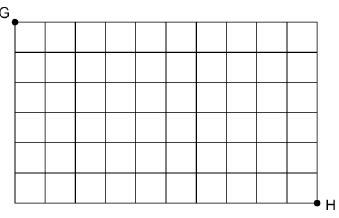
\includegraphics[width=0.25\textwidth]{chemin_court.png}

Chaque bloc est un carré de 100 m sur 100 m. On cherche d'abord la longueur minimal en se déplaçant sur les segments:
\begin{itemize}
\item Comment faut-il se déplacer sur ce quadrillage
si on ne veut pas dépasser la longueur minimale ?
\item  Combien de déplacement pour la longueur minimale ?
\item  Combien de trajets différents y a-t-il
pour aller de la gare à l'hôtel avec cette longueur minimale ?
\end{itemize}
\begin{Correction}
\begin{itemize}
\item aller soit à droite soit vers le bas. Si on va gauche, le trajet se rallonge de deux car il faudra compenser en allant une fois à droite. Idem pour vers le haut 
\item 16 déplacements par exemple aller 10 fois à droite puis 6 fois vers le bas
\item On pose B = "vers le bas" et D = "vers la droite". Un exemple de chemin de G à H est le mot
BD...DBB...B où B est écrit 6 fois et D est écrit 10 fois. Le nombre de chemins cherché est clairement le
nombre d'anagrammes du mot précédent. Si on regarde la position du D dans un anagramme, on se ramène à un triage sans remise et sans ordre.
Donc le nombre de chemins est 6 parmi 16, soit $\begin{pmatrix}
16\\6
\end{pmatrix}$
\end{itemize}
\end{Correction}

\end{Exercice}
\begin{Exercice}[rangement]
Mr T a 5 livres d'algèbre, 3 livres de géométrie et 4 livres d'analyse.
\begin{enumerate}
\item De combien de manières peut-il les ranger sur une étagère de sa bibliothèque ?
\item Même question en les regroupant par sujet.
\end{enumerate}
\begin{Correction}
\begin{enumerate}
\item Un rangement correspond à un tirage sans remise et avec ordre de toutes les boules (le numéro de la boule correspond à la position du livre). Soit $12!$.
\item nombre de regroupant par sujet="rangement par matière, puis rangement de chaque matière". Soit $3!5!3!4!$.
\end{enumerate}
\end{Correction}

\end{Exercice}
\begin{Exercice}[Nombre de parties d'un ensemble]
Dénombrer  l'ensemble des parties de $\Intf{1}{n}$, noté $ \mathcal{P}(\Intf{1}{n})$. 
\begin{Correction}
Démontrons que cette fonction est bijective :
\[
f:
  \begin{array}{rcl}
    \mathcal{P}(\Intf{1}{n}) & \longrightarrow & \mathcal{F}(\Intf{1}{n},\{0,1\}) \\
      A & \longmapsto & \mathbf 1_A \\
  \end{array}
\]avec $\mathbf 1_A$ fonction indicatrice de l'ensemble $A$
\[
\mathbf 1_A :\begin{array}{rcl}  \Intf{1}{n} & \longrightarrow & \{0,1\}  \\
i & \longmapsto & \left\{\begin{matrix}  1 \ \mbox{si} \ i \ \in \ A \\ 0 \ \mbox{si} \ i \ \notin \ A \end{matrix}\right. \end{array}
\]
\begin{itemize}
\item \textit{injective }: soit $A,B\in \mathcal{P}(\Intf{1}{n})$ tel que $f(A)=f(B)$, d'où $\mathbf 1_A=\mathbf 1_B$ donc $A=B$.
\item \textit{surjectivité} : soit $\phi\in  \mathcal{F}(\Intf{1}{n},\{0,1\})$. On pose $A=\{i\in \Intf{1}{n}:\phi(i)=1\}$. on a bien $f(A)=\phi$.
\end{itemize}
Comme $f$ est bijective $\text{Card}(\mathcal{P}(\Intf{1}{n}))=\text{Card}(\mathcal{F}(\Intf{1}{n},\{0,1\}))=2^n$.
\end{Correction}

\end{Exercice}
\end{document}
